\documentclass[a4paper]{article}
\usepackage[pdftex]{hyperref}
\usepackage[latin1]{inputenc}
\usepackage[english]{babel}
\usepackage{a4wide}
\usepackage{amsmath}
\usepackage{amssymb}
\usepackage{algorithmic}
\usepackage{algorithm}
\usepackage{ifthen}
\usepackage{listings}
% move the asterisk at the right position
\lstset{basicstyle=\ttfamily,tabsize=4,literate={*}{${}^*{}$}1}
%\lstset{language=C,basicstyle=\ttfamily}
\usepackage{moreverb}
\usepackage{palatino}
\usepackage{multicol}
\usepackage{tabularx}
\usepackage{comment}
\usepackage{verbatim}
\usepackage{color}

%% pdflatex?
\newif\ifpdf
\ifx\pdfoutput\undefined
\pdffalse % we are not running PDFLaTeX
\else
\pdfoutput=1 % we are running PDFLaTeX
\pdftrue
\fi
\ifpdf
\usepackage[pdftex]{graphicx}
\else
\usepackage{graphicx}
\fi
\ifpdf
\DeclareGraphicsExtensions{.pdf, .jpg}
\else
\DeclareGraphicsExtensions{.eps, .jpg}
\fi

\parindent=0cm
\parskip=0cm

\setlength{\columnseprule}{0.4pt}
\addtolength{\columnsep}{2pt}

\addtolength{\textheight}{5.5cm}
\addtolength{\topmargin}{-26mm}
\pagestyle{empty}

%%
%% Sheet setup
%% 
\newcommand{\coursename}{Machine Learning}
\newcommand{\courseno}{CO22-320372}
 
\newcommand{\sheettitle}{Homework}
\newcommand{\mytitle}{}
\newcommand{\mytoday}{{April 15th}, 2018}

% Current Assignment number
\newcounter{assignmentno}
\setcounter{assignmentno}{8}

% Current Problem number, should always start at 1
\newcounter{problemno}
\setcounter{problemno}{1}

%%
%% problem and bonus environment
%%
\newcounter{probcalc}
\newcommand{\problem}[2]{
  \pagebreak[2]
  \setcounter{probcalc}{#2}
  ~\\
  {\large \textbf{Problem {\arabic{assignmentno}}.{\arabic{problemno}}} \hspace{0.2cm}\textit{#1}} \refstepcounter{problemno}\vspace{2pt}\\}

\newcommand{\bonus}[2]{
  \pagebreak[2]
  \setcounter{probcalc}{#2}
  ~\\
  {\large \textbf{Bonus Problem \textcolor{blue}{\arabic{assignmentno}}.\textcolor{blue}{\arabic{problemno}}} \hspace{0.2cm}\textit{#1}} \refstepcounter{problemno}\vspace{2pt}\\}

%% some counters  
\newcommand{\assignment}{\arabic{assignmentno}}

%% solution  
\newcommand{\solution}{\pagebreak[2]{\bf Solution:}\\}

%% Hyperref Setup
\hypersetup{pdftitle={Homework \assignment},
  pdfsubject={\coursename},
  pdfauthor={},
  pdfcreator={},
  pdfkeywords={Machine Learning},
  %pdfpagemode={FullScreen},
  %colorlinks=true,
  %bookmarks=true,
  %hyperindex=true,
  bookmarksopen=false,
  bookmarksnumbered=true,
  breaklinks=true,
  %urlcolor=darkblue
  urlbordercolor={0 0 0.7}
}

\begin{document}
\coursename \hfill Course: \courseno\\
Jacobs University Bremen \hfill \mytoday\\
{Zihan Qi \& Danni Long}\hfill
\vspace*{0.3cm}\\
\begin{center}
{\Large \sheettitle{} {\assignment}\\}
\end{center}

\section*{Procedure}
First, We took first 100 vectors from each class as \textbf{train data}, and save the rest 100 from each class as \textbf{test data}.\\\\
 We did \textbf{PCA} for dimension reduction. Since the dimension of patterns ($N$ = 1000) is much larger than the dimension of space(240), we choose our $k$ to be 240, as identity operator. (We also tried set precision of dimension reduction to be 99.5\%, then we get k to be 170) Through \textbf{SVD}, U as a 240 * 240 is our matrix for further operation in Linear regression.\\\\
 Then, we add padding for reducted train data, and we created a 1000 * 10 matrix Z. Every 100 rows stand for the same class, which has 1 at corresponding position, and 0 at rest.\\\\
 Next, we compute \textbf{$W_{opt}$} through the projection of all train data onto U matrix, using its transpose as matrix \textbf{$\Phi$}, and project Z onto the subspace $\Phi$ formed, which is the smallest distance from Z to the space. That is our optimal decision function $W_{opt}$.\\\\
 Next, We compute the \textbf{mean square error}, and \textbf{misclassification rate} through a loop on all train data, using MAX Ind to find the index of max value of current vector, while using find command to locate the supposed current class, and compare them, if not equal, number of misclassification add 1. We went through the whole loop, then compute how much misclassification in total data.\\\\
 Next, start testing. In a large loop for the feature K to be 1,2...240. Then U matrix will vary from containing only U1, to U1 U2, till full U.(also padding one as bias in the last) Mapping new data onto varying U, Using the same $W_{opt}$ we have from previous to compute test error. Then the rests are similar as before.\\
\newpage
\section*{Observation}
\textbf{Linear Scaling:}\\\\
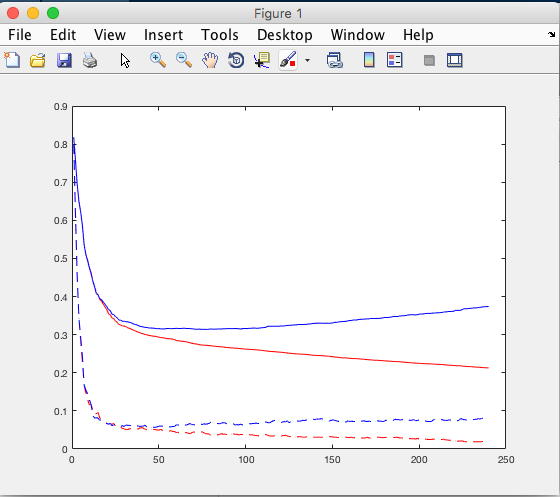
\includegraphics[width=5in]{LinearScaling.png}\\\\
\textbf{Logarithmic Scaling:}\\\\
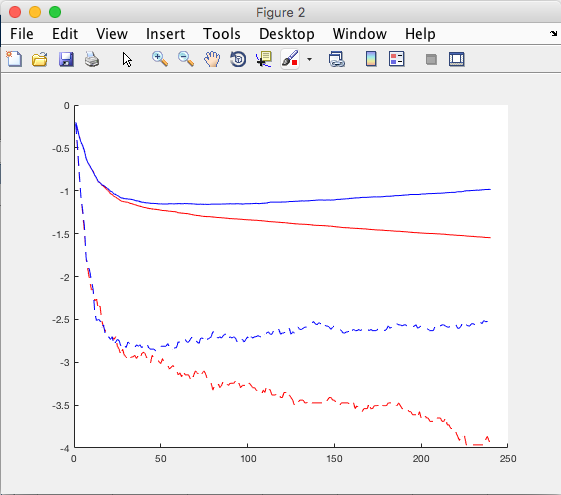
\includegraphics[width=5in]{LogScaling.png}\\
MSE train: solid red\\
MSE test: solid blue\\
MISS train: dashed red\\
MISS test: dashed blue\\

\newpage
\section*{Discussion}
We could tell from the graph, the train error is drastic decreasing from beginning, and gradually converge to 0. However, the test data has reach its minimum around K = 40, then it starts to increasing once again. Then 40 will be our optimal value to get the max correct classification. if we took K $<$ 40, at very left, this would be a underfitting problem, which may mean that this kind of classification can not meet the user's requirement, and couldn't really tell the characteristics of data. This Model is too inflexible. If K is chosen to be much larger than 40, it is a overfitting problem, which means this model is too flexible, later on using on test data, it will lead to terrible misclassification. We actually use the case when K = 170, since we tried data reduction precision to be 99\%, and get m = 170 in Matrix U. It is a bit better than the case K = 240, but still a overfitting problem.
 \end{document}
